\newpage
\section[Фигура 2]{Фигура 2}

Строим квадрат, дважды дублируем.

Матрицы преобразований для построения верхней грани:
\begin{equation*}
    A_{top} = 
    \begin{pmatrix}
        0.707&  0.707& 0\\ 
        -0.707&  0.707& 0\\ 
        0&  0& 1
    \end{pmatrix} \hspace{24pt}
    B_{top} = 
    \begin{pmatrix} 
        1&  0& 0\\
        0&  0.5& 0\\
        0&  0& 1
    \end{pmatrix} \hspace{24pt}
    C_{top} = 
    \begin{pmatrix}
        1&  0& 0\\ 
        0&  1& 200\\ 
        0&  0& 1
    \end{pmatrix}
\end{equation*}


Матрицы преобразований для построения левой грани:
\begin{equation*}
    A_{left} = 
    \begin{pmatrix}
         0.707& 0& 0\\ 
         0& 1& 0\\ 
         0&  0& 1
    \end{pmatrix} \hspace{24pt}
    B_{left} = 
    \begin{pmatrix} 
        1& 0& 0\\
        0& 1& 100\\
        0& 0& 1
    \end{pmatrix} \hspace{24pt}
    C_{left}= 
    \begin{pmatrix}
        1&  0& 0\\ 
        -0.5&  1& 100\\ 
        0&  0& 1
    \end{pmatrix}
\end{equation*}

Далее дублируем левую грань, 
применяем преобразования к дубликату для получения правой грани:
\begin{equation*}
    A_{right} = 
    \begin{pmatrix}
         -1& 0& 0\\ 
         0& 1& 0\\ 
         0&  0& 1
    \end{pmatrix} \hspace{24pt}
    B_{right} = 
    \begin{pmatrix} 
        1& 0& 141.4\\
        0& 1& 0\\
        0& 0& 1
    \end{pmatrix} \hspace{24pt}
\end{equation*}

Результирующие матрицы:
\begin{equation*}
    M_{top} = C_{top}\times B_{top}\times A_{top} = 
    \begin{pmatrix} 
        0.707& 0.707& 0\\
        -0.353& 0.353& 200\\
        0& 0& 1
    \end{pmatrix} \hspace{24pt}
\end{equation*}

\begin{equation*}
    M_{left} = C_{left}\times B_{left}\times A_{left} = 
    \begin{pmatrix} 
        0.707& 0& 0\\
        -0.353& 1& 100\\
        0& 0& 1
    \end{pmatrix} \hspace{24pt}
\end{equation*}

\begin{equation*}
    M_{right} = B_{right}\times A_{right} = 
    \begin{pmatrix} 
        -1& 0& 141.4\\
        0& 1& 0\\
        0& 0& 1
    \end{pmatrix} \hspace{24pt}
\end{equation*}

*$M_{right}$ \textit{ применяется к копии левой грани}

\newpage
Ниже приведены этапы применения изменений:
\begin{figure}[H]
    \begin{minipage}[h]{0.27\linewidth}
        \center{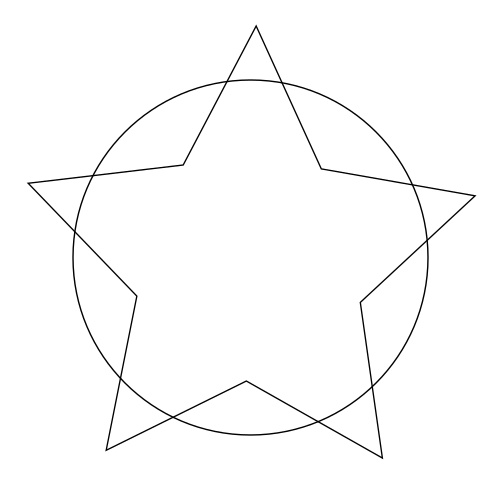
\includegraphics[width=1\linewidth]{2_1_create.png}}\\
        Создание фигур
    \end{minipage}
    \hfill
    \begin{minipage}[h]{0.27\linewidth}
        \center{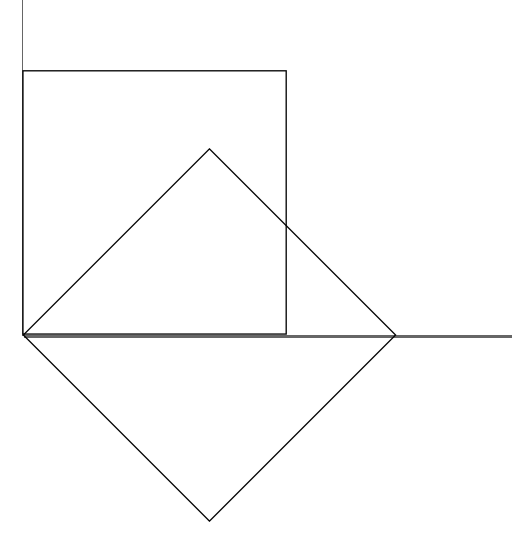
\includegraphics[width=1\linewidth]{2_2_rotate.png}}\\
        $A_{top}$ (поворот)
    \end{minipage}
    \hfill
    \begin{minipage}[h]{0.27\linewidth}
        \center{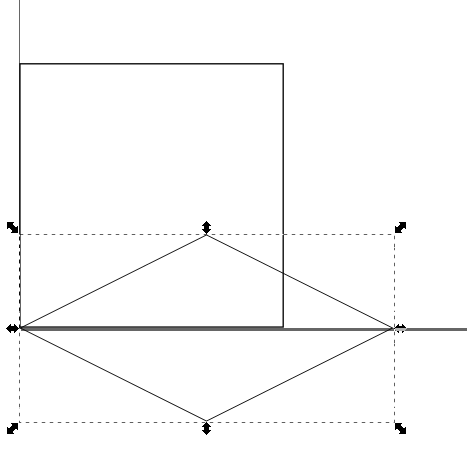
\includegraphics[width=1\linewidth]{2_3_scale.png}}\\
        $B_{top}$ (сжатие)
    \end{minipage}
    \vfill
    \vspace{12pt}
    \begin{minipage}[h]{0.27\linewidth}
        \center{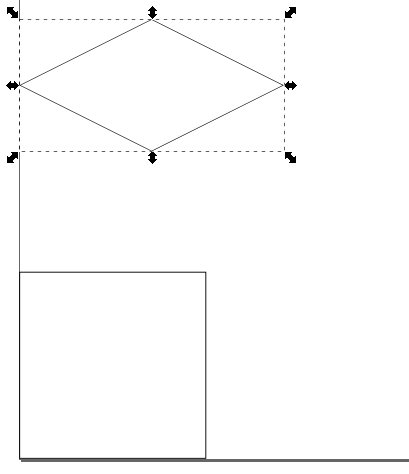
\includegraphics[width=1\linewidth]{2_4_move.png}}\\
        $C_{top}$ (перемещение)
    \end{minipage}
    \hfill
    \begin{minipage}[h]{0.27\linewidth}
        \center{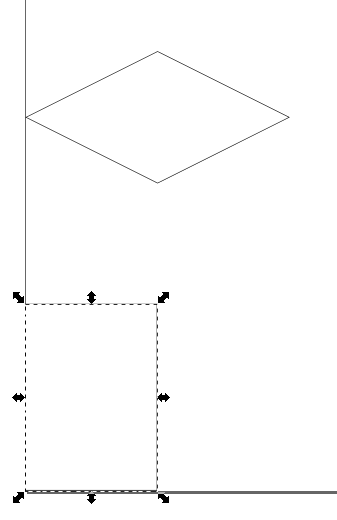
\includegraphics[width=1\linewidth]{2_5_scale.png}}\\
        $A_{left}$ (сжатие)
    \end{minipage}
    \hfill
    \begin{minipage}[h]{0.27\linewidth}
        \center{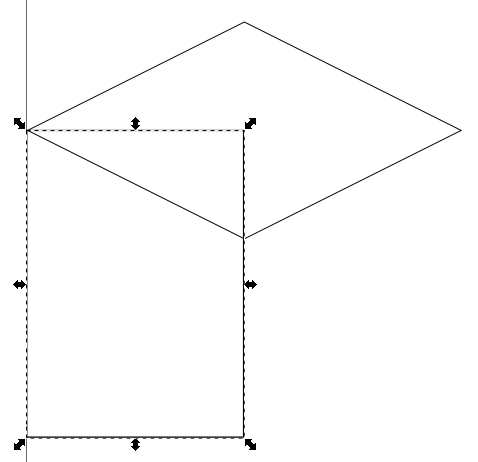
\includegraphics[width=1\linewidth]{2_6_move.png}}\\
        $B_{left}$ (перемещение)
    \end{minipage}
    \vfill
    \vspace{12pt}
    \begin{minipage}[h]{0.27\linewidth}
        \center{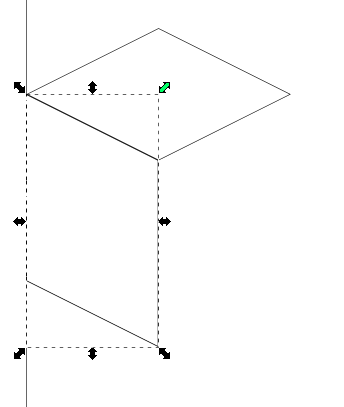
\includegraphics[width=1\linewidth]{2_7_skew.png}}\\
        $C_{left}$ (скос)
    \end{minipage}
    \hfill
    \begin{minipage}[h]{0.27\linewidth}
        \center{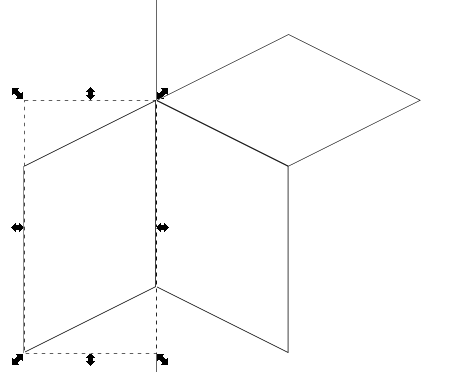
\includegraphics[width=1\linewidth]{2_8_mirror.png}}\\
        $A_{right}$ (отражение)
    \end{minipage}
    \hfill
    \begin{minipage}[h]{0.27\linewidth}
        \center{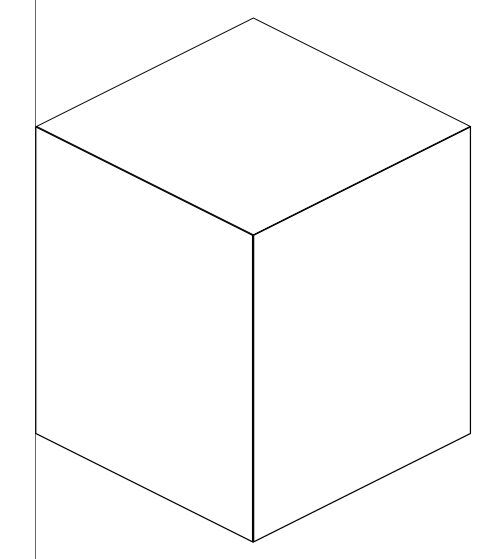
\includegraphics[width=1\linewidth]{2_9_move.png}}\\
        $B_{right}$ (перемещение)
    \end{minipage}
\end{figure}
